\documentclass[12pt,letterpaper]{article}
\usepackage{fullpage}
\usepackage[top=2cm, bottom=4.5cm, left=2.5cm, right=2.5cm]{geometry}
\usepackage{amsmath,amsthm,amsfonts,amssymb,amscd}
\usepackage{lastpage}
\usepackage{enumerate}
\usepackage{fancyhdr}
\usepackage{mathrsfs}
\usepackage{xcolor}
\usepackage{fancyvrb}
\usepackage{graphicx}
\usepackage{listings}
\usepackage{float}
\usepackage{hyperref}
\usepackage{tikz}
\usepackage{relsize}
\usepackage{fancyvrb}
\usepackage{multirow}
\usepackage{booktabs}
\usepackage{import}
\usetikzlibrary{shapes.geometric,fit}

\hypersetup{%
  colorlinks=true,
  linkcolor=blue,
  linkbordercolor={0 0 1}
}

\setlength{\parindent}{0.0in}
\setlength{\parskip}{0.05in}

\theoremstyle{definition}
\newtheorem*{statement}{Statement}
\newtheorem*{claim}{Claim}
\newtheorem*{theorem}{Theorem}
\newtheorem*{lemma}{Lemma}

\newcommand{\contra}{\Rightarrow\!\Leftarrow}
\newcommand{\R}{\mathbb{R}}
\newcommand{\F}{\mathbb{F}}
\newcommand{\Z}{\mathbb{Z}}
\newcommand{\Zeq}{\mathbb{Z}_{\geq 0}}
\newcommand{\Zg}{\mathbb{Z}_{>0}}
\newcommand{\Req}{\mathbb{R}_{\geq 0}}
\newcommand{\Rg}{\mathbb{R}_{>0}}
\newcommand{\N}{\mathbb{N}}
\newcommand{\Q}{\mathbb{Q}}
\newcommand{\C}{\mathbb{C}}
\DeclareMathOperator{\Cov}{Cov}
\DeclareMathOperator{\Var}{Var}

\newcommand{\incfig}[1] {%
    \import{./figures/}{#1.pdf_tex}
}

\graphicspath{ {./figures/} }

\title{ECON 3412 HW 5}
\author{David Chen, dc3451}

\begin{document}

\maketitle

\section*{Problem 1}

\subsection*{a}

We simply load the data into \verb|R| directly, no need to demarcate it as panel data:
\begin{Verbatim}[fontsize=\small]
> library(haven)
> library(plm)
> demo <- read_dta("./income_democracy.dta")
\end{Verbatim}
To check if it is balanced:
\begin{Verbatim}[fontsize=\small]
> is.pbalanced(demo)
[1] FALSE
\end{Verbatim}
which means we are missing some observation for some entity at some time; for example, Afghanistan is missing $log\_gdppc$ for all of the years in the data set.

\subsection*{b}

For the US in 1965, the democracy index is 0.92.
\begin{Verbatim}[fontsize=\small]
> demo$dem_ind[demo$country == "United States" & demo$year == 1965]
[1] 0.92
\end{Verbatim}

For Uruguay in 1965, the democracy index is 1.
\begin{Verbatim}[fontsize=\small]
> demo$dem_ind[demo$country == "Uruguay" & demo$year == 1965]
[1] 1
\end{Verbatim}

For Trinidad and Tobago in 1995, the democracy index is 1.
\begin{Verbatim}[fontsize=\small]
> demo$dem_ind[demo$country == "Trinidad and Tobago" & demo$year == 1995]
[1] 1
\end{Verbatim}

For Venezuela in 1995, the democracy index is $0.67$.
\begin{Verbatim}[fontsize=\small]
> demo$dem_ind[demo$country == "Venezuela, RB" & demo$year == 1995]
[1] 0.6666667
\end{Verbatim}

\subsection*{c}

I assume this question means for all years and all countries. In that case, the desired data and statistics are gotten as follows:
\begin{Verbatim}[fontsize=\small]
> mean(demo$dem_ind, na.rm = TRUE)
[1] 0.4990732
> sd(demo$dem_ind, na.rm = TRUE)
[1] 0.3713367
> quantile(demo$dem_ind, c(0, 0.10, 0.25, 0.50, 0.75, 0.90, 1), na.rm = TRUE)
       0%       10%       25%       50%       75%       90%      100%
0.0000000 0.0000000 0.1666667 0.5000000 0.8333333 1.0000000 1.0000000
\end{Verbatim}
so a mean of $0.4991$, standard deviation of $0.3713$, max 1, min 0, and quantiles as shown above.

\subsection*{d}

As an aside, \verb|R|'s clubSandwich package and STATA have different implementations of clustered errors, with STATA making some finite sample adjustment (as far as I can tell from the documentation) so making the correction to the covariance matrix of the regression of $(m (N-1)) / [(m - 1)(N - p)]$, where $m$ is the number of clusters, $N$ is the total number of observations, and $p$ is the number of covariates \textit{seems} to align \verb|R| with STATA on the regressions done on the lecture slides, so if my numbers are a little off, this is probably why. (The biggest divergence I can find in this set is I think on Q2, part g, where the SEs are misaligned by <1\%)

We get that the appropriate \verb|R| to mimic \verb|reg dem_ind log_gdppc, vce(cluster code)| is
\begin{Verbatim}[fontsize=\small]
> dem_gdp_nofe <- lm(dem_ind ~ log_gdppc, data = demo)
> coef_test(dem_gdp_nofe, vcov = "CR1S", cluster = demo$code)
        Coef. Estimate     SE t-stat d.f. p-val (Satt) Sig.
1 (Intercept)   -1.355 0.1004  -13.5 71.0       <0.001  ***
2   log_gdppc    0.236 0.0118   19.9 69.9       <0.001  ***
\end{Verbatim}

\subsection*{e}

The coefficient of $log\_gdppc$ is $0.236$, and is significantly different from 0 at $p < 0.001$. This means that there is a statistically significant (positive) relationship between gdp/capita and the presence of democracy in a country. Quantitatively, we should, expect to see an average increase of about $0.01(0.236) = 0.00236$ in the democracy index in a country for every percent change in gdp/capita.

\subsection*{f}

Then, from above, a 20\% change in gdp/capita would predict on average an increase in the democracy index of $20(0.00236) = 0.0472 $. The 95\% confidence interval for the coefficient was $0.236 \pm (1.96 \cdot 0.0118) = (.212, .259)$, so we have that on the lower bound, the prediction would be $20(0.01)(0.212) = 0.0424$ and on the upper bound, the prediction becomes $20(0.01)(0.259) = 0.0518$, so an appropriate interval is an increase in somewhere inside of $(0.0424, 0.0518)$ for a 20\% increase in the gdp/capita.

\subsection*{g}

The \verb|R| equivalent to \verb|xtreg dem_ind log_gdppc, fe vce(cluster code)| is
\begin{Verbatim}[fontsize=\small]
> dem_gdp <- plm(dem_ind ~ log_gdppc, data = demo,
                 index = c("country", "year"), model = "within")
> coef_test(dem_gdp, vcov = "CR1S", cluster = demo$code)

      Coef. Estimate     SE t-stat d.f. p-val (Satt) Sig.
1 log_gdppc   0.0837 0.0315   2.66 49.7       0.0106    *
\end{Verbatim}
so a much lower estimate of the effect of $log\_gdppc$ than before.

\subsection*{h}

I use the following \verb|R|:
\begin{Verbatim}[fontsize=\small]
> demo$y60 <- as.integer(demo$year == 1960)
> demo$y65 <- as.integer(demo$year == 1965)
> demo$y70 <- as.integer(demo$year == 1970)
> demo$y75 <- as.integer(demo$year == 1975)
> demo$y80 <- as.integer(demo$year == 1980)
> demo$y85 <- as.integer(demo$year == 1985)
> demo$y90 <- as.integer(demo$year == 1990)
> demo$y95 <- as.integer(demo$year == 1995)
> dem_gdp_time <- plm(dem_ind ~ log_gdppc + y60 + y65 + y70 + y75 +
                   y80 + y85 + y90 + y95, data = demo,
                 index = c("country", "year"), model = "within")
> coef_test(dem_gdp, vcov = "CR1S", cluster = demo$code)

      Coef. Estimate     SE t-stat  d.f. p-val (Satt) Sig.
1 log_gdppc   0.0536 0.0424  1.264  44.5      0.21296
2   y60TRUE  -0.0324 0.0432 -0.749  75.5      0.45589
3   y65TRUE  -0.0321 0.0389 -0.827  73.0      0.41119
4   y70TRUE  -0.1592 0.0380 -4.194  86.0      < 0.001  ***
5   y75TRUE  -0.1801 0.0346 -5.206  97.9      < 0.001  ***
6   y80TRUE  -0.1302 0.0338 -3.854 110.7      < 0.001  ***
7   y85TRUE  -0.1195 0.0301 -3.974 119.2      < 0.001  ***
8   y90TRUE  -0.0745 0.0243 -3.071 122.9      0.00263   **
9   y95TRUE  -0.0228 0.0139 -1.646 126.0      0.10224
\end{Verbatim}

\section*{Problem 2}

\subsection*{a}

\subsubsection*{i}

Using OLS,
\begin{Verbatim}[fontsize=\small]
reg <- read_dta("./deregulate.dta")
reg$lnvc <- log(reg$vc)
reg$lnpl <- log(reg$pl)
reg$lnpf <- log(reg$pf)
reg$lnpm <- log(reg$pm)
reg$lnstage <- log(reg$stage)
ols_reg <- robust_lm(lnvc ~ reg + year + lnpl + lnpf + lnpm + lnstage, data = reg)
ols_reg[[2]]

t test of coefficients:

             Estimate Std. Error t value Pr(>|t|)
(Intercept) -5.619307   3.286938 -1.7096  0.08853 .
reg         -0.104425   0.141993 -0.7354  0.46274
year        -0.068819   0.051587 -1.3340  0.18336
lnpl         0.913703   0.439856  2.0773  0.03875 *
lnpf        -0.419206   0.236140 -1.7752  0.07702 .
lnpm         1.673207   0.896546  1.8663  0.06312 .
lnstage      1.319770   0.051129 25.8126  < 2e-16 ***
---
Signif. codes:  0 ‘***’ 0.001 ‘**’ 0.01 ‘*’ 0.05 ‘.’ 0.1 ‘ ’ 1
\end{Verbatim}

\subsubsection*{ii}

Using fixed effect regressions and robust standard errors,
\begin{Verbatim}[fontsize=\small]
> fe_reg <- plm(lnvc ~ reg + year + lnpl + lnpf + lnpm + lnstage, data = reg,
                index = c("airline", "year"), model = "within")
> coeftest(fe_reg, vcov = vcovHC(fe_reg, type = "sss"))
t test of coefficients:

         Estimate Std. Error t value  Pr(>|t|)
reg     -0.010389   0.035193 -0.2952  0.768088
year     0.045823   0.014722  3.1125  0.002081 **
lnpl     0.129390   0.138641  0.9333  0.351619
lnpf     0.088011   0.078256  1.1247  0.261862
lnpm     0.383767   0.188518  2.0357  0.042883 *
lnstage  0.863640   0.185214  4.6629 5.187e-06 ***
---
Signif. codes:  0 ‘***’ 0.001 ‘**’ 0.01 ‘*’ 0.05 ‘.’ 0.1 ‘ ’ 1
\end{Verbatim}

On piazza they said to use normal standard errors, so
\begin{Verbatim}[fontsize=\small]
> summary(fe_reg)
Coefficients:
         Estimate Std. Error t-value  Pr(>|t|)
reg     -0.010389   0.040427 -0.2570 0.7974109
year     0.045823   0.013071  3.5058 0.0005435 ***
lnpl     0.129390   0.101310  1.2772 0.2027831
lnpf     0.088011   0.060380  1.4576 0.1462598
lnpm     0.383767   0.261833  1.4657 0.1440466
lnstage  0.863640   0.061097 14.1355 < 2.2e-16 ***
---
Signif. codes:  0 ‘***’ 0.001 ‘**’ 0.01 ‘*’ 0.05 ‘.’ 0.1 ‘ ’ 1
\end{Verbatim}

\subsubsection*{iii}

Using fixed effects and robust clustered standard errors,
\begin{Verbatim}[fontsize=\small]
## coeftest and coef_test are implemented in different packages,
## and as such have different names.
> coef_test(fe_reg, vcov = "CR1S", cluster = reg$airline)
    Coef. Estimate     SE t-stat  d.f. p-val (Satt) Sig.
1     reg  -0.0104 0.0352 -0.295 16.77      0.77145
2    year   0.0458 0.0147  3.113 15.55      0.00689   **
3    lnpl   0.1294 0.1386  0.933  6.86      0.38235
4    lnpf   0.0880 0.0783  1.125 17.98      0.27553
5    lnpm   0.3838 0.1885  2.036 17.27      0.05742    .
6 lnstage   0.8636 0.1852  4.663 11.26      < 0.001  ***
---
Signif. codes:  0 ‘***’ 0.001 ‘**’ 0.01 ‘*’ 0.05 ‘.’ 0.1 ‘ ’ 1
\end{Verbatim}

\subsection*{b}

The regulation dummy's coefficient is interpreted as the difference between the logarithm of the variable cost when it was regulated and the logarithm of the variable cost when it wasn't regulated keeping all other things in the regression including factors heterogeneous across firms equal. In particular, we should expect that transitioning from regulation to deregulation ($reg = 1$ to $reg  = 0$) actually changes variable costs by about a factor of $1/(1 + \beta_{reg})$ (equivalent to the statement that variable costs lowered by $100\beta_{reg}\%$ moving from $reg = 0$ to $reg = 1$) where $\beta_{reg}$ is the coefficient of $reg$ in the regression (in particular this is an increase of $\beta_{reg}$ since $\beta_{reg} < 0$ for all the above regressions).
% \[
%   \log(vc \mid reg = 1) - \log(vc \mid reg = 0) =  0.0501 \implies \log\left(\frac{vc \mid reg = 1}{vc \mid reg = 0}\right) = 0.0501
% \]
% and using the $\log$ approximation close to $1$, we have that $\frac{(vc \mid reg = 1) - (vc \mid reg = 0)}{vc \mid reg 0} \approx 0.0501$ or
% \[
%   (vc \mid reg = 1) \approx 1.0501 (vc \mid reg = 0) \implies 0.952(vc \mid reg = 1) = (vc \mid reg = 0)
% \]
% so we have that the removal of regulations decreased variable costs by about 5\%.

\subsection*{c}

The interpretation of year in this regression is that for every passing year, all else held equal, we should expect to see the variable costs of an airline to increase by a factor of about $1 + \beta_{year}$ where $\beta_{year}$ is the coefficient of year in the regression.

\subsection*{d}

We should expect the variance of the OLS estimators to be larger when the variance in the sample data is larger. In particular, if we have that we just naively use OLS, we have that different firms operate on different scales, and as a result, we probably have a high amount of variance in the data, since variable costs are lower in smaller firms; controlling for factors heterogeneous across the firms strengthens the relationship between the regressors and the dependent variable, reducing error.

We care about clustered errors specifically in this case exactly because of the above: the factors here, such as the pricing of materials or the average length of a flight are likely to be correlated within a firm: if a firm has shorter flights one year, we would expect it to have shorter flights in the next year since decisions such as the type of flights to make (domestic vs international, for example) are determined often by the structure of the firm, so there is likely autocorrelation within an entity.

\subsection*{e}

It actually shows that since $\beta_{reg} = -0.01 < 0$ in the fixed effects regression with clustered errors, that the transition between regulation to deregulation actually increased variable costs by about $1\%$.

\subsection*{f}

The important aspect here is that technology change in airlines, as a monolithic industry with heavy testing and regulation, is probably fairly smooth and not sudden. As a result, we can expect that technological change is constant and positive over any given year, meaning that including $year$ in the regression should control for technical improvements. Of course, in the case of sudden technological change, the control is inadequate, but this is unlikely to be the case in a industry with high stocks of capital and slow phase in of new tech. As a result, we can use the coefficient of $reg$ to check the effect of regulation on variable costs without concern for the effects technical change masking the effects of regulation.

\subsection*{g}

\begin{Verbatim}[fontsize=\small]
fe_reg <- plm(lnvc ~ reg + year + lnpl + lnpf + lnpm + lnstage +
                I(lnpl^2) + I(lnpf^2) + I(lnpm^2) + I(lnstage^2), data = reg,
              index = c("airline", "obs"), model = "within")
coef_test(fe_reg, vcov = "CR1S", cluster = reg$airline)
          Coef. Estimate     SE  t-stat  d.f. p-val (Satt) Sig.
1           reg   0.0523 0.0262  1.9990 15.13      0.06391    .
2          year   0.0466 0.0304  1.5331 18.76      0.14193
3          lnpl   0.1602 0.1621  0.9886  6.63      0.35755
4          lnpf   0.0103 0.2514  0.0408 17.24      0.96789
5          lnpm  -5.0493 7.1996 -0.7013 18.21      0.49197
6       lnstage   1.4327 1.3522  1.0595 11.94      0.31034
7     I(lnpl^2)  -0.4498 0.1328 -3.3867  8.41      0.00887   **
8     I(lnpf^2)  -0.0179 0.0671 -0.2674 18.23      0.79220
9     I(lnpm^2)   0.5262 0.7534  0.6984 18.15      0.49378
10 I(lnstage^2)  -0.0527 0.1140 -0.4620 12.03      0.65233
\end{Verbatim}

The fact that the coefficient of $lnpl^2$ is signiticantly nonzero ($|t| > 2.57 \implies p < 0.01$) means that we missed some important nonlinearity in our original regression, and that this suggests that the conclusions made in e are not quite accurate. In particular, after including the squares, the sign of $reg$ changes and is significant at a 5\% ($|t| > 1.96$) level now, signaling that the transition to deregulation actually lowered variable costs by about $5\%$.

\subsection*{h}
\begin{Verbatim}[fontsize=\small]
> linearHypothesis(fe_reg, c("I(lnpl^2) = 0", "I(lnpf^2) = 0",
                             "I(lnpm^2) = 0", "I(lnstage^2) = 0"),
                   vcov = vcovCR(fe_reg, type = "CR1S", cluster = reg$airline),
                   test = "F")
Linear hypothesis test

Hypothesis:
I(lnpl^2) = 0
I(lnpf^2) = 0
I(lnpm^2) = 0
I(lnstage^2) = 0

Model 1: restricted model
Model 2: lnvc ~ reg + year + lnpl + lnpf + lnpm + lnstage + I(lnpl^2) +
    I(lnpf^2) + I(lnpm^2) + I(lnstage^2)

Note: Coefficient covariance matrix supplied.

  Res.Df Df      F    Pr(>F)
1    239
2    235  4 6.0277 0.0001238 ***
---
Signif. codes:  0 ‘***’ 0.001 ‘**’ 0.01 ‘*’ 0.05 ‘.’ 0.1 ‘ ’ 1
\end{Verbatim}

This gives the correct $F-$statistic, but is tested against the wrong degree of freedom since the function is unaware of the fixed effects regression. Manually testing the $F$-statistic on $4$ and $22$ degrees of freedom, \verb|pf(6.02, 4, 22) = 0.998|, so they are jointly significant at $p = 0.02$.

\subsection*{i}

If we make the following (reasonable) assumptions, namely that more efficient flight times are either shorter or longer, but not both, and that deregulation doesn't massively change the destinations and locations of flights, then $lnstage$ already controls for this effect (since more efficient flight paths would directly be reflected in minutes flown on an average flight under these assumptions), since it is a measure of the average length of the airline’s flights that year. This would mean that the conclusions drawn by e and g are still unchanged.

However, it's not 100\% clear that more efficient flight paths are shorter flight paths; in particular, one might envision that sometimes longer flight times are more efficient when eliminating small stops, such that a flight that goes DC $\rightarrow$ LA is more efficient than one that goes DC $\rightarrow$ OKC $\rightarrow$ LA, but on the other hand, some flights might be more efficient as smaller times, i.e. a flight that now can fly a tighter/shorter route due to removal of regulations. In this case, the relationship between efficiency and $stage$ is not sufficient to control for this effect in the regression. In particular, efficiency might increase, but since this means both more shorter and longer flights, $stage$ is unchanged. In this case, the internal validity of e and g is threatened due to omitted variable bias.

\section*{Problem 3}

\subsection*{a}

We do the following:
\begin{Verbatim}[fontsize=\small]
> q <- read_dta("./q.dta")
> naive <- robust_lm(ikb ~ qb, q)
> naive[[2]]
t test of coefficients:

             Estimate Std. Error t value  Pr(>|t|)
(Intercept) 0.1091277  0.0017290  63.118 < 2.2e-16 ***
qb          0.0158021  0.0013608  11.612 < 2.2e-16 ***
---
Signif. codes:  0 ‘***’ 0.001 ‘**’ 0.01 ‘*’ 0.05 ‘.’ 0.1 ‘ ’ 1
\end{Verbatim}

The sign is positive and the magnitude of the coefficient of $qb$ is 0.0158, so we have that for every unit increase in $qb$, we expect to see on average an increase in $ikb$ of 0.0158. Qualitatively, this means that the more valued the firm is in the market relative to their book value, the higher investment they enjoy, after normalizing the amount of investment by the amount of capital they already own.

We cannot give this a causal interpretation; in particular, there are lots of omitted variables at play here. For example, a variable that varies between firms but not time might be the age of the firms; a old company like Boeing might have a lot more capital in long-term assets than a newer one like spaceX, simply because they've been around for longer and thus a lower $ikb$, and older companies might have a $q \approx 1$, but newer firms might be overhyped and thus have $q > 1$, so this is an omitted variable. Similarly, a factor varying across time but not firm is general economic outlook: if we're in a recession, investors are pessimistic, and then $q$ lowers since market valuations lower, and $ikb$ lowers since investment lowers.

\subsection*{b}

Fixed effect regression:
\begin{Verbatim}[fontsize=\small]
> fe_reg_q <- plm(ikb ~ qb, data = q, index = c("cusip", "year"), model = "within")
> coef_test(fe_reg_q, vcov = "CR1S", cluster = q$cusip)
  Coef. Estimate      SE t-stat d.f. p-val (Satt) Sig.
1    qb   0.0202 0.00337      6 26.6       <0.001  ***
\end{Verbatim}

Entity demeaned regression:
\begin{Verbatim}[fontsize=\small]
> q$qb_d <- 0
> q$ikb_d <- 0
> for (i in 1:length(q[[1]])) {
    q$ikb_d[i] = q$ikb[i] - mean(q$ikb[q$cusip == q$cusip[i]])
    q$qb_d[i] = q$qb[i] - mean(q$qb[q$cusip == q$cusip[i]])
  }
> ent_demean <- lm(ikb_d ~ qb_d, data = q)
> coef_test(ent_demean, vcov = "CR1S", cluster = q$cusip)
        Coef. Estimate       SE t-stat  d.f. p-val (Satt) Sig.
1 (Intercept) 1.21e-18 6.05e-19      2 187.0       0.0464    *
2        qb_d 2.02e-02 3.37e-03      6  26.6       <0.001  ***
\end{Verbatim}

so we see that the estimate of the corefficient of $qb$ comes out the same as $0.0202$ with a standard error of $0.00337$, as desired.

In both cases, the coefficient has actually increased from $0.015$ to $0.02$, so this suggests that the omitted factors that varied across firms (but not time) were actually negatively correlated with $qb$ and the omitted factors were positively correlated with $ikb$ (or positively correlated with $qb$ and negatively correlated with $ikb$), since this regression shows that the effect of $q$ was underestimated before.

\subsection*{c}
\subsubsection*{a}

\begin{figure}[H]
  \begin{center}
    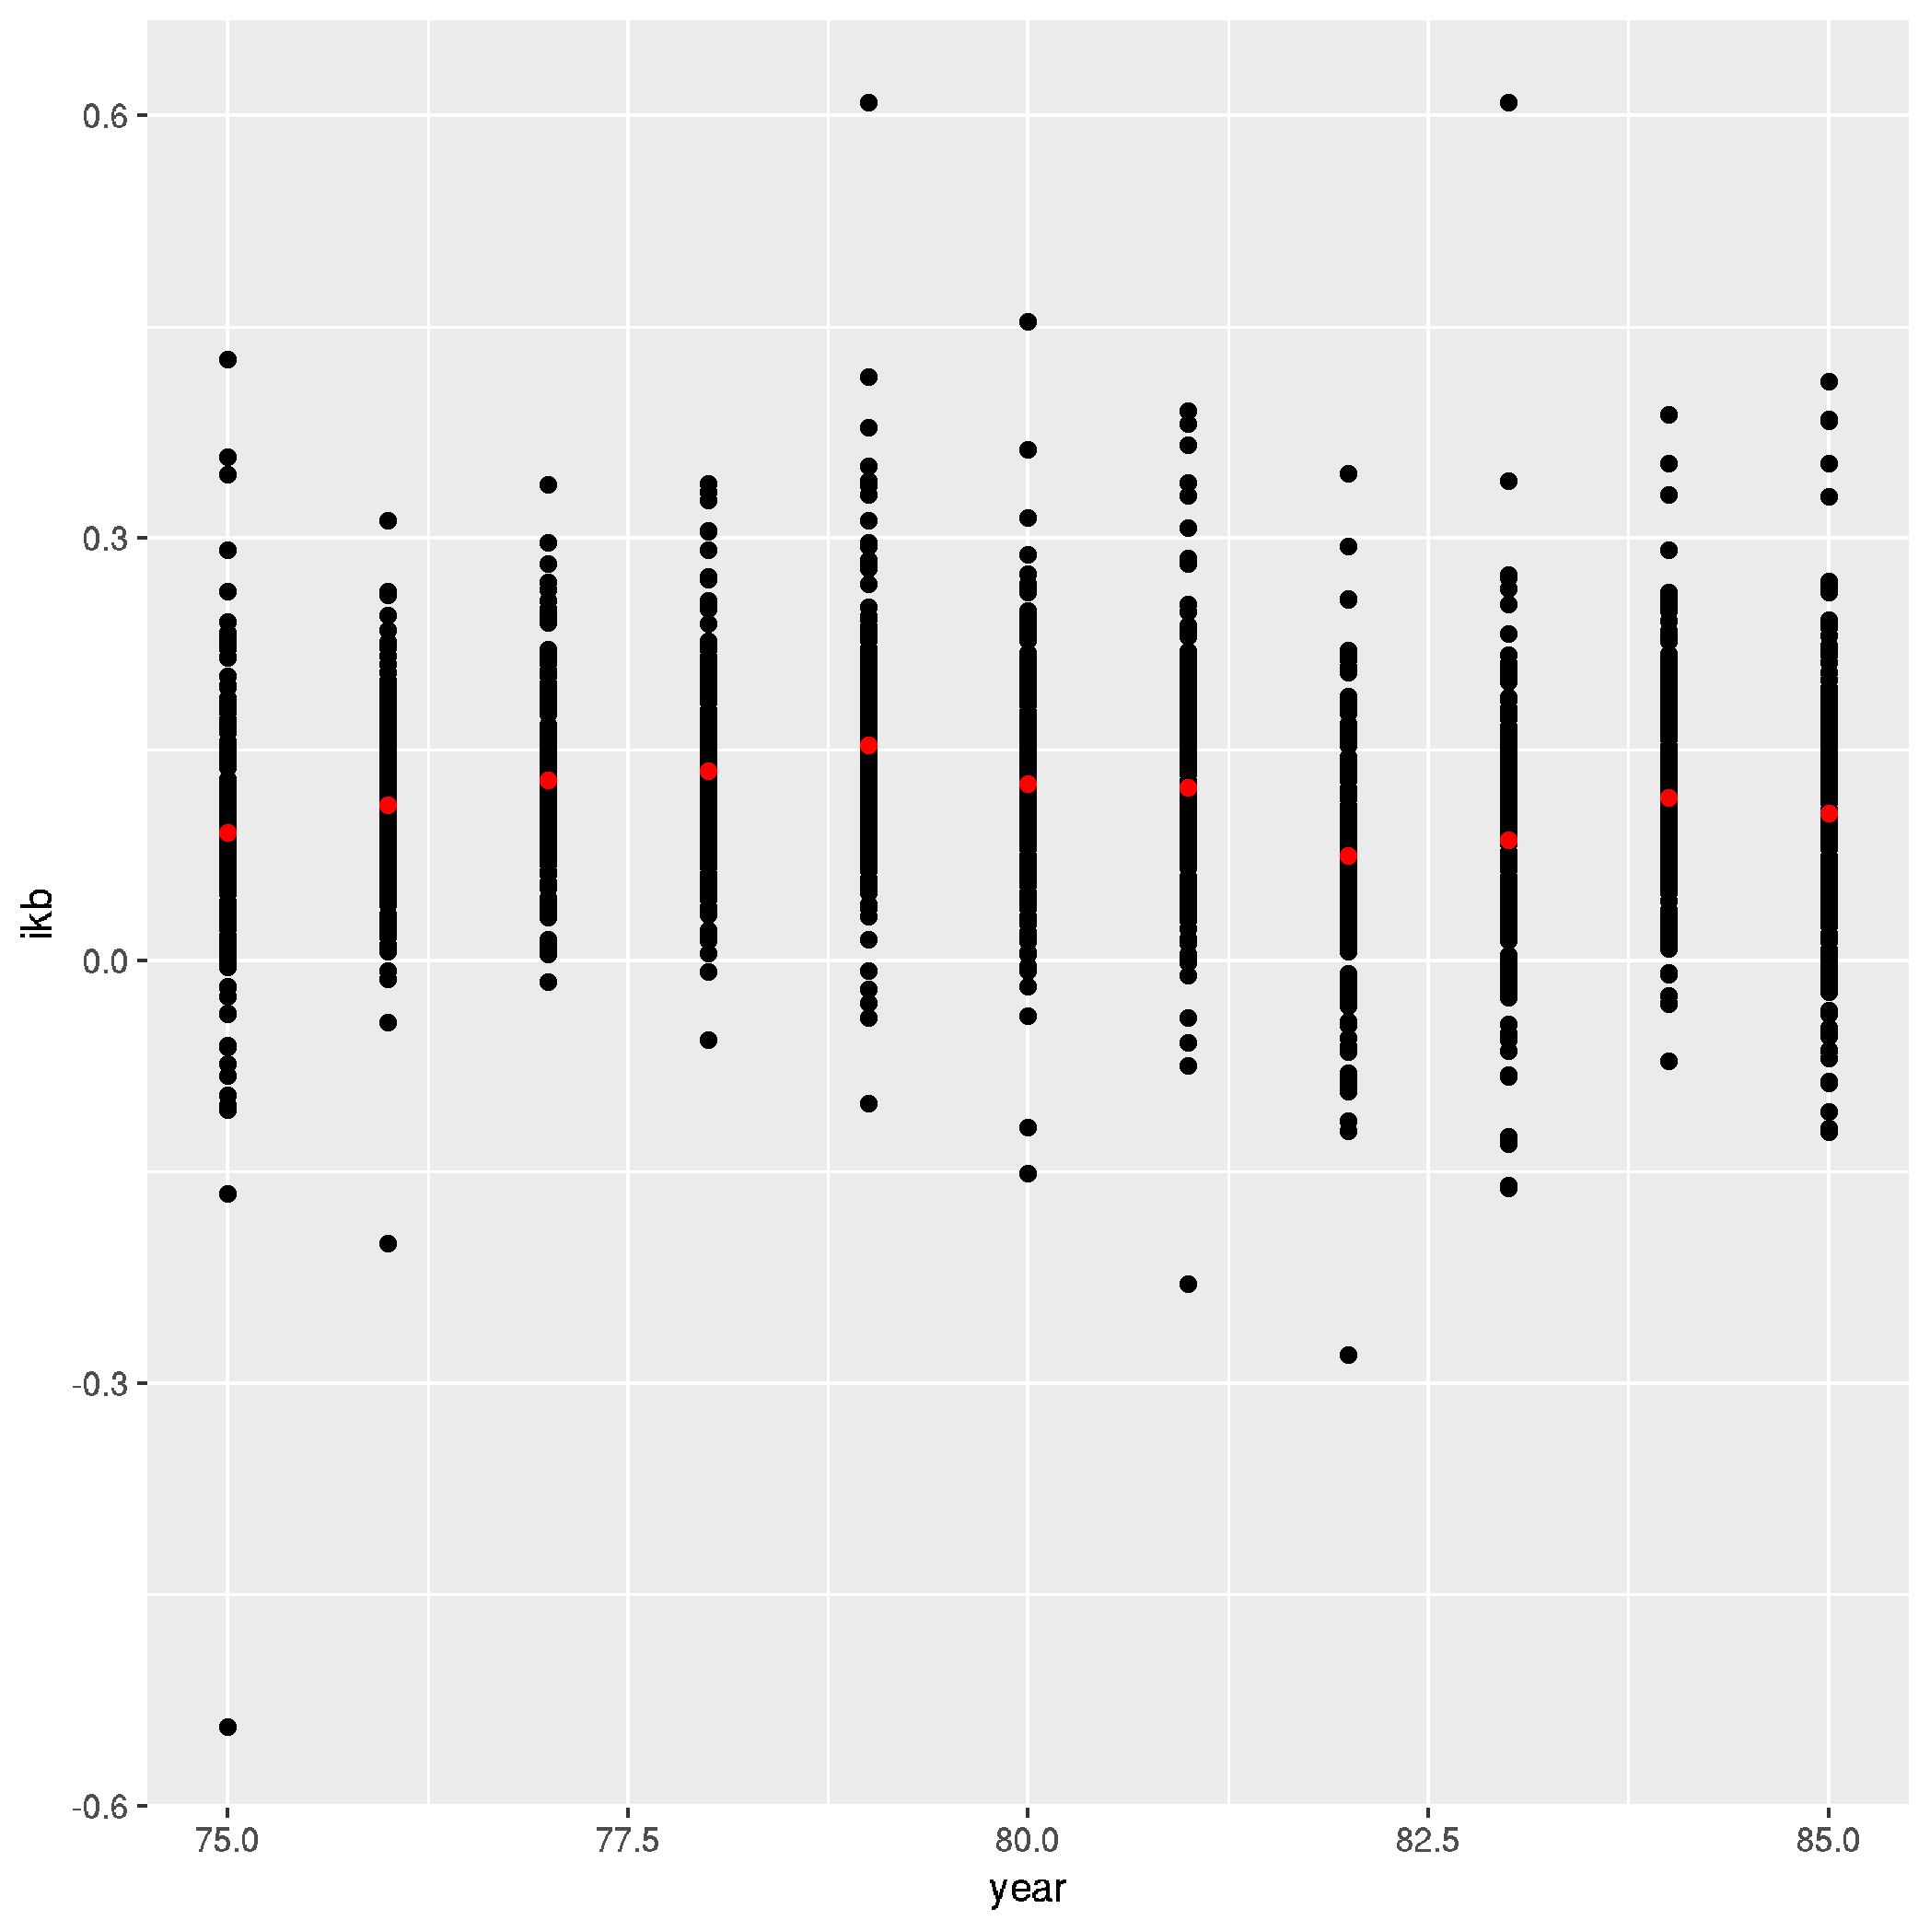
\includegraphics[width=10cm]{all.png}
    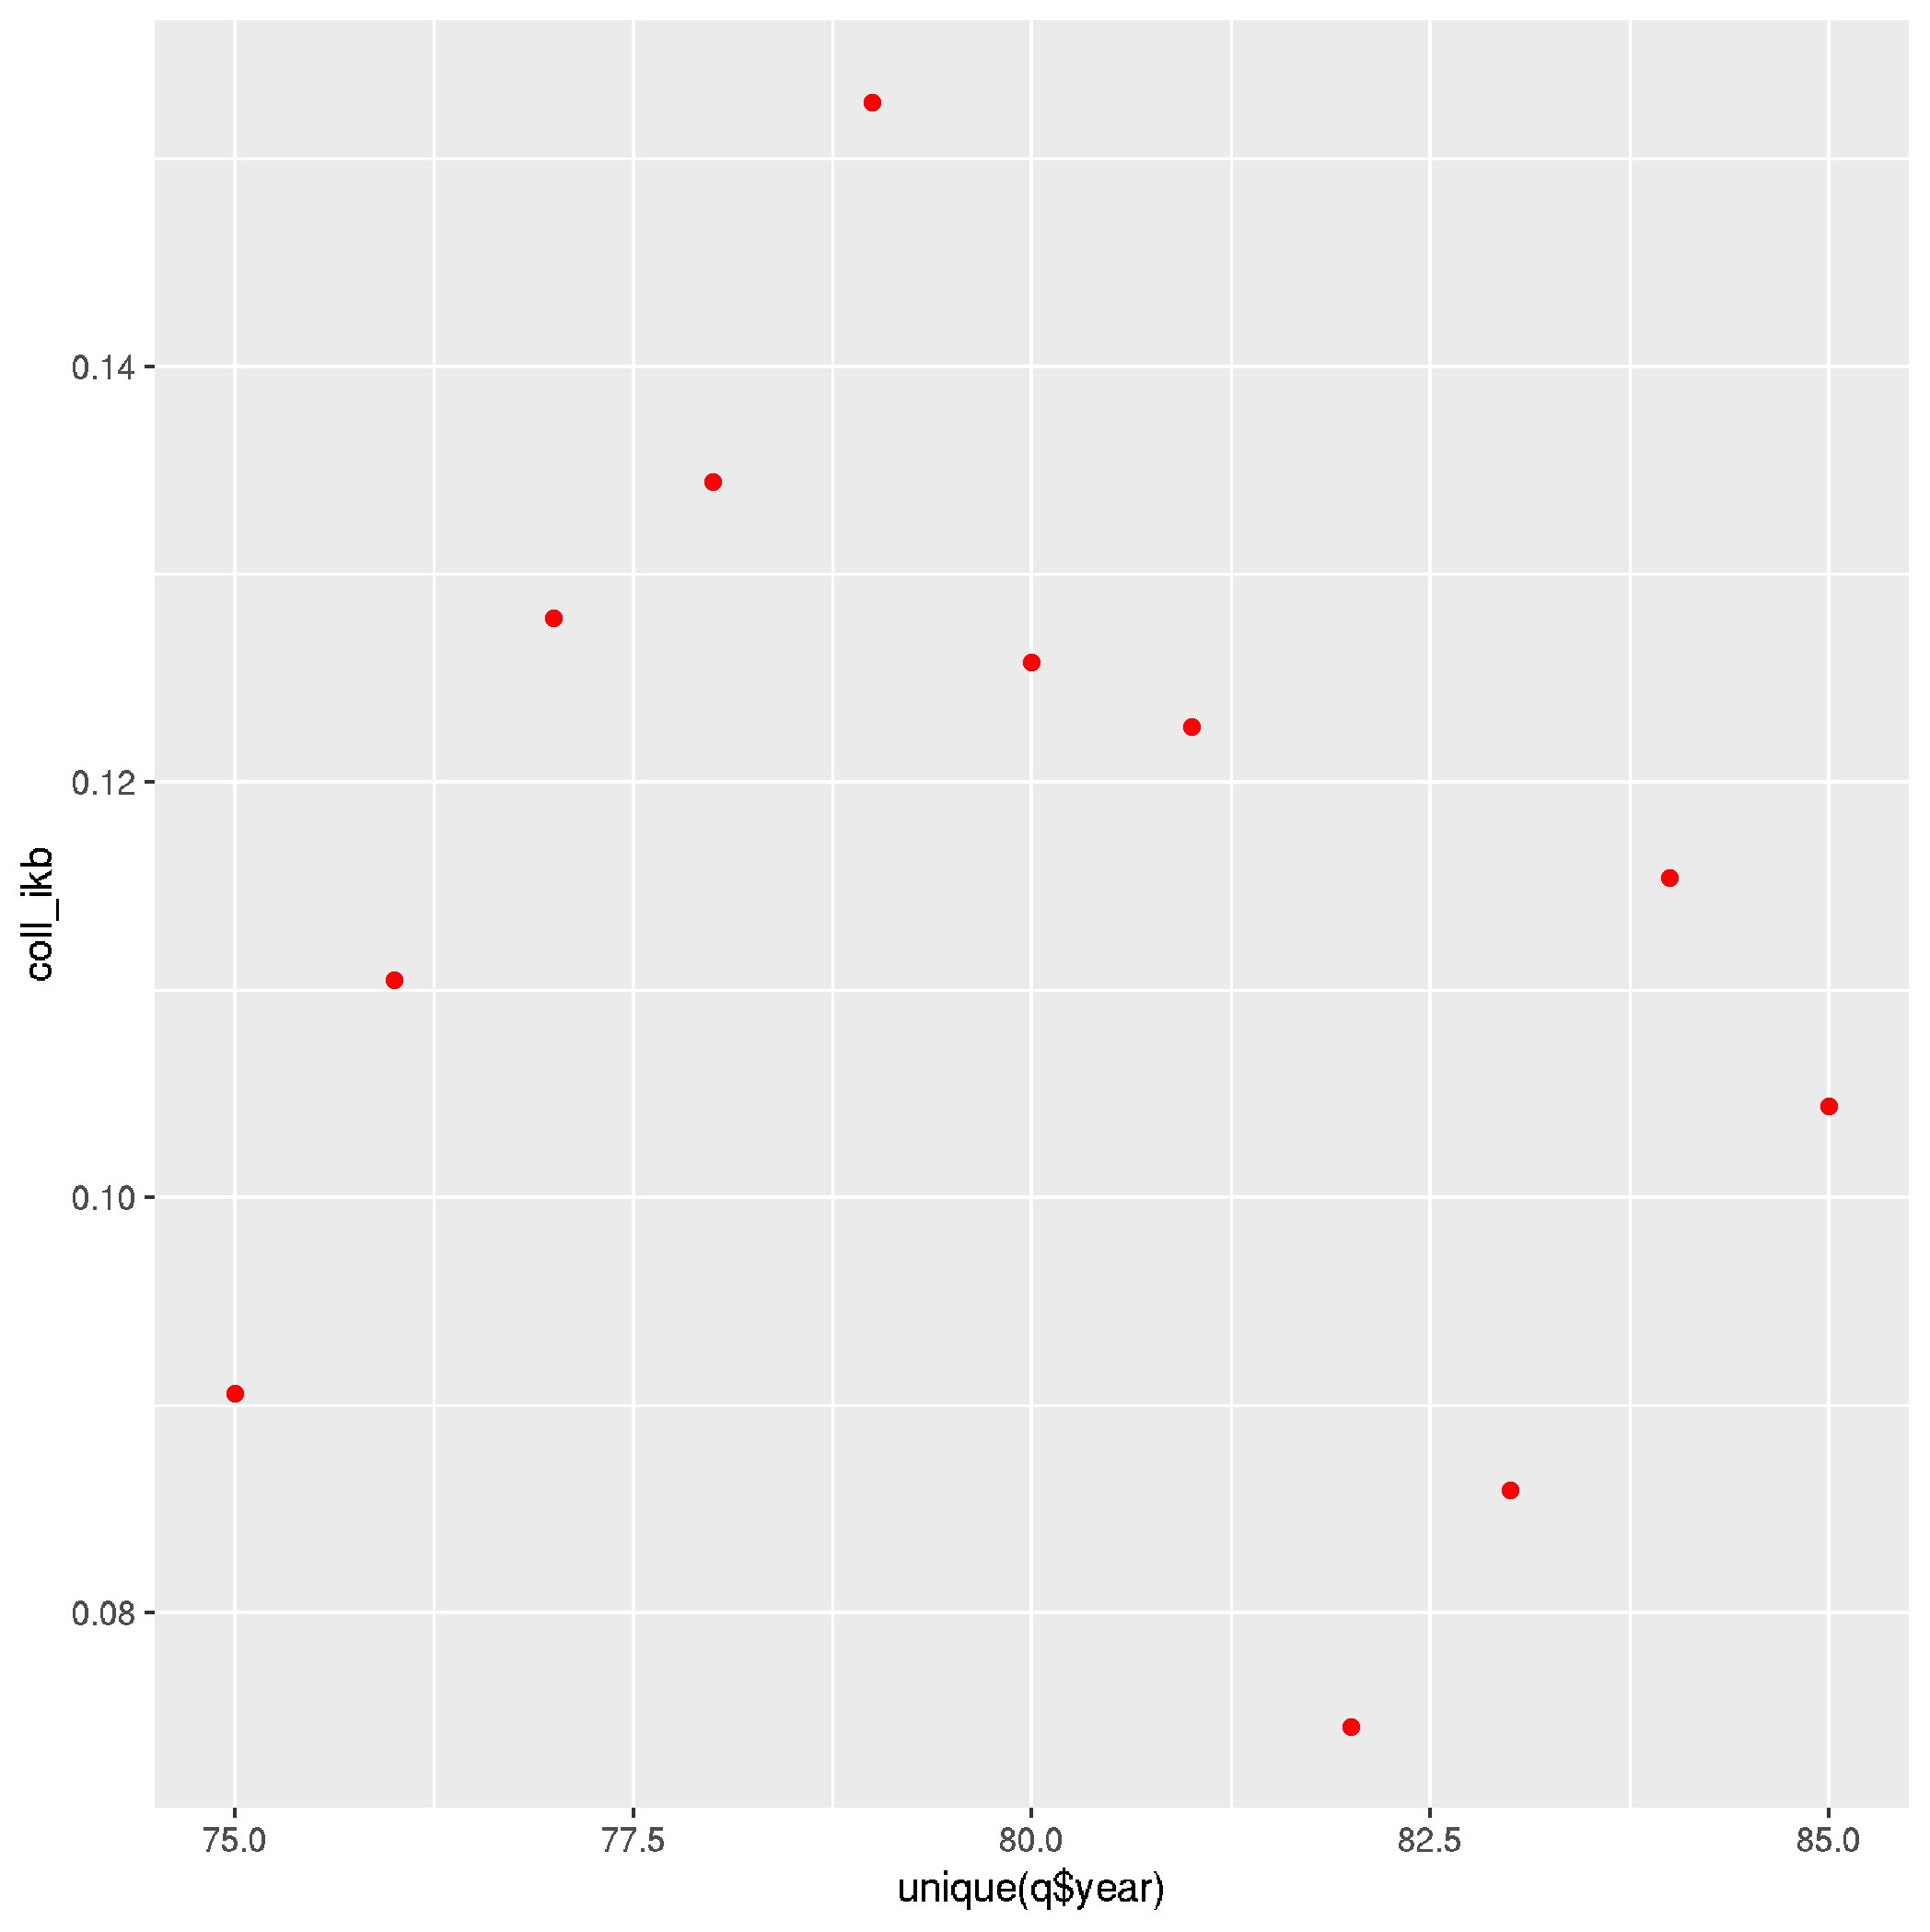
\includegraphics[width=10cm]{coll.png}
  \end{center}
\end{figure}

The top figure is a graph of all $ikb$ data points plotted against the year of observation; the red dots are the means of the $ikb$ observations in any one year; the bottom graph is just the means.

\begin{Verbatim}[fontsize=\small]
> ggplot() + geom_point(data = q, aes(x = year, y = ikb)) +
             geom_point(aes(x = unique(q$year), y = coll_ikb), color = "red")
> ggplot() + geom_point(aes(x = unique(q$year), y = coll_ikb), color = "red")
\end{Verbatim}

\subsubsection*{b}

Regression after creating the requisite time dummies:
\begin{Verbatim}[fontsize=\small]
> q$y75 = as.integer(q$year == 75)
> q$y76 = as.integer(q$year == 76)
> q$y77 = as.integer(q$year == 77)
> q$y78 = as.integer(q$year == 78)
> q$y79 = as.integer(q$year == 79)
> q$y80 = as.integer(q$year == 80)
> q$y81 = as.integer(q$year == 81)
> q$y82 = as.integer(q$year == 82)
> q$y83 = as.integer(q$year == 83)
> q$y84 = as.integer(q$year == 84)
> q$y85 = as.integer(q$year == 85)
> fe_reg_time_q <- plm(ikb ~ qb + y75 + y76 + y78 + y79 + y80 + y81 +
                             y82 + y83 + y84,
                       data = q, index = c("cusip", "year"), model = "within")
> coef_test(fe_reg_time_q, vcov = "CR1S", cluster = q$cusip)
   Coef.  Estimate      SE  t-stat  d.f. p-val (Satt) Sig.
1     qb  2.01e-02 0.00317  6.3378  24.7      < 0.001  ***
2    y75 -2.17e-02 0.00711 -3.0506 186.5      0.00262   **
3    y76 -6.69e-03 0.00489 -1.3680 187.0      0.17294
4    y78  2.21e-02 0.00541  4.0936 186.9      < 0.001  ***
5    y79  4.32e-02 0.00649  6.6576 186.3      < 0.001  ***
6    y80  1.58e-02 0.00636  2.4807 186.3      0.01400    *
7    y81  1.00e-02 0.00652  1.5422 186.6      0.12471
8    y82 -3.29e-02 0.00642 -5.1259 185.0      < 0.001  ***
9    y83 -2.48e-02 0.00616 -4.0239 186.4      < 0.001  ***
10   y84 -9.26e-05 0.00492 -0.0188 187.0      0.98501
\end{Verbatim}

A plot of the coefficient of each year, with the coef on the y and the year on the x:
\begin{Verbatim}[fontsize=\small]
> effects = c(0.01953, -0.03018, -0.01504,  0.01366,  0.03467,
              0.00723,  0.00158, -0.04153, -0.03331, -0.00849, -0.01675)
> ggplot() + geom_point(aes(x = years, y = effects))
\end{Verbatim}

\begin{figure}[H]
  \begin{center}
    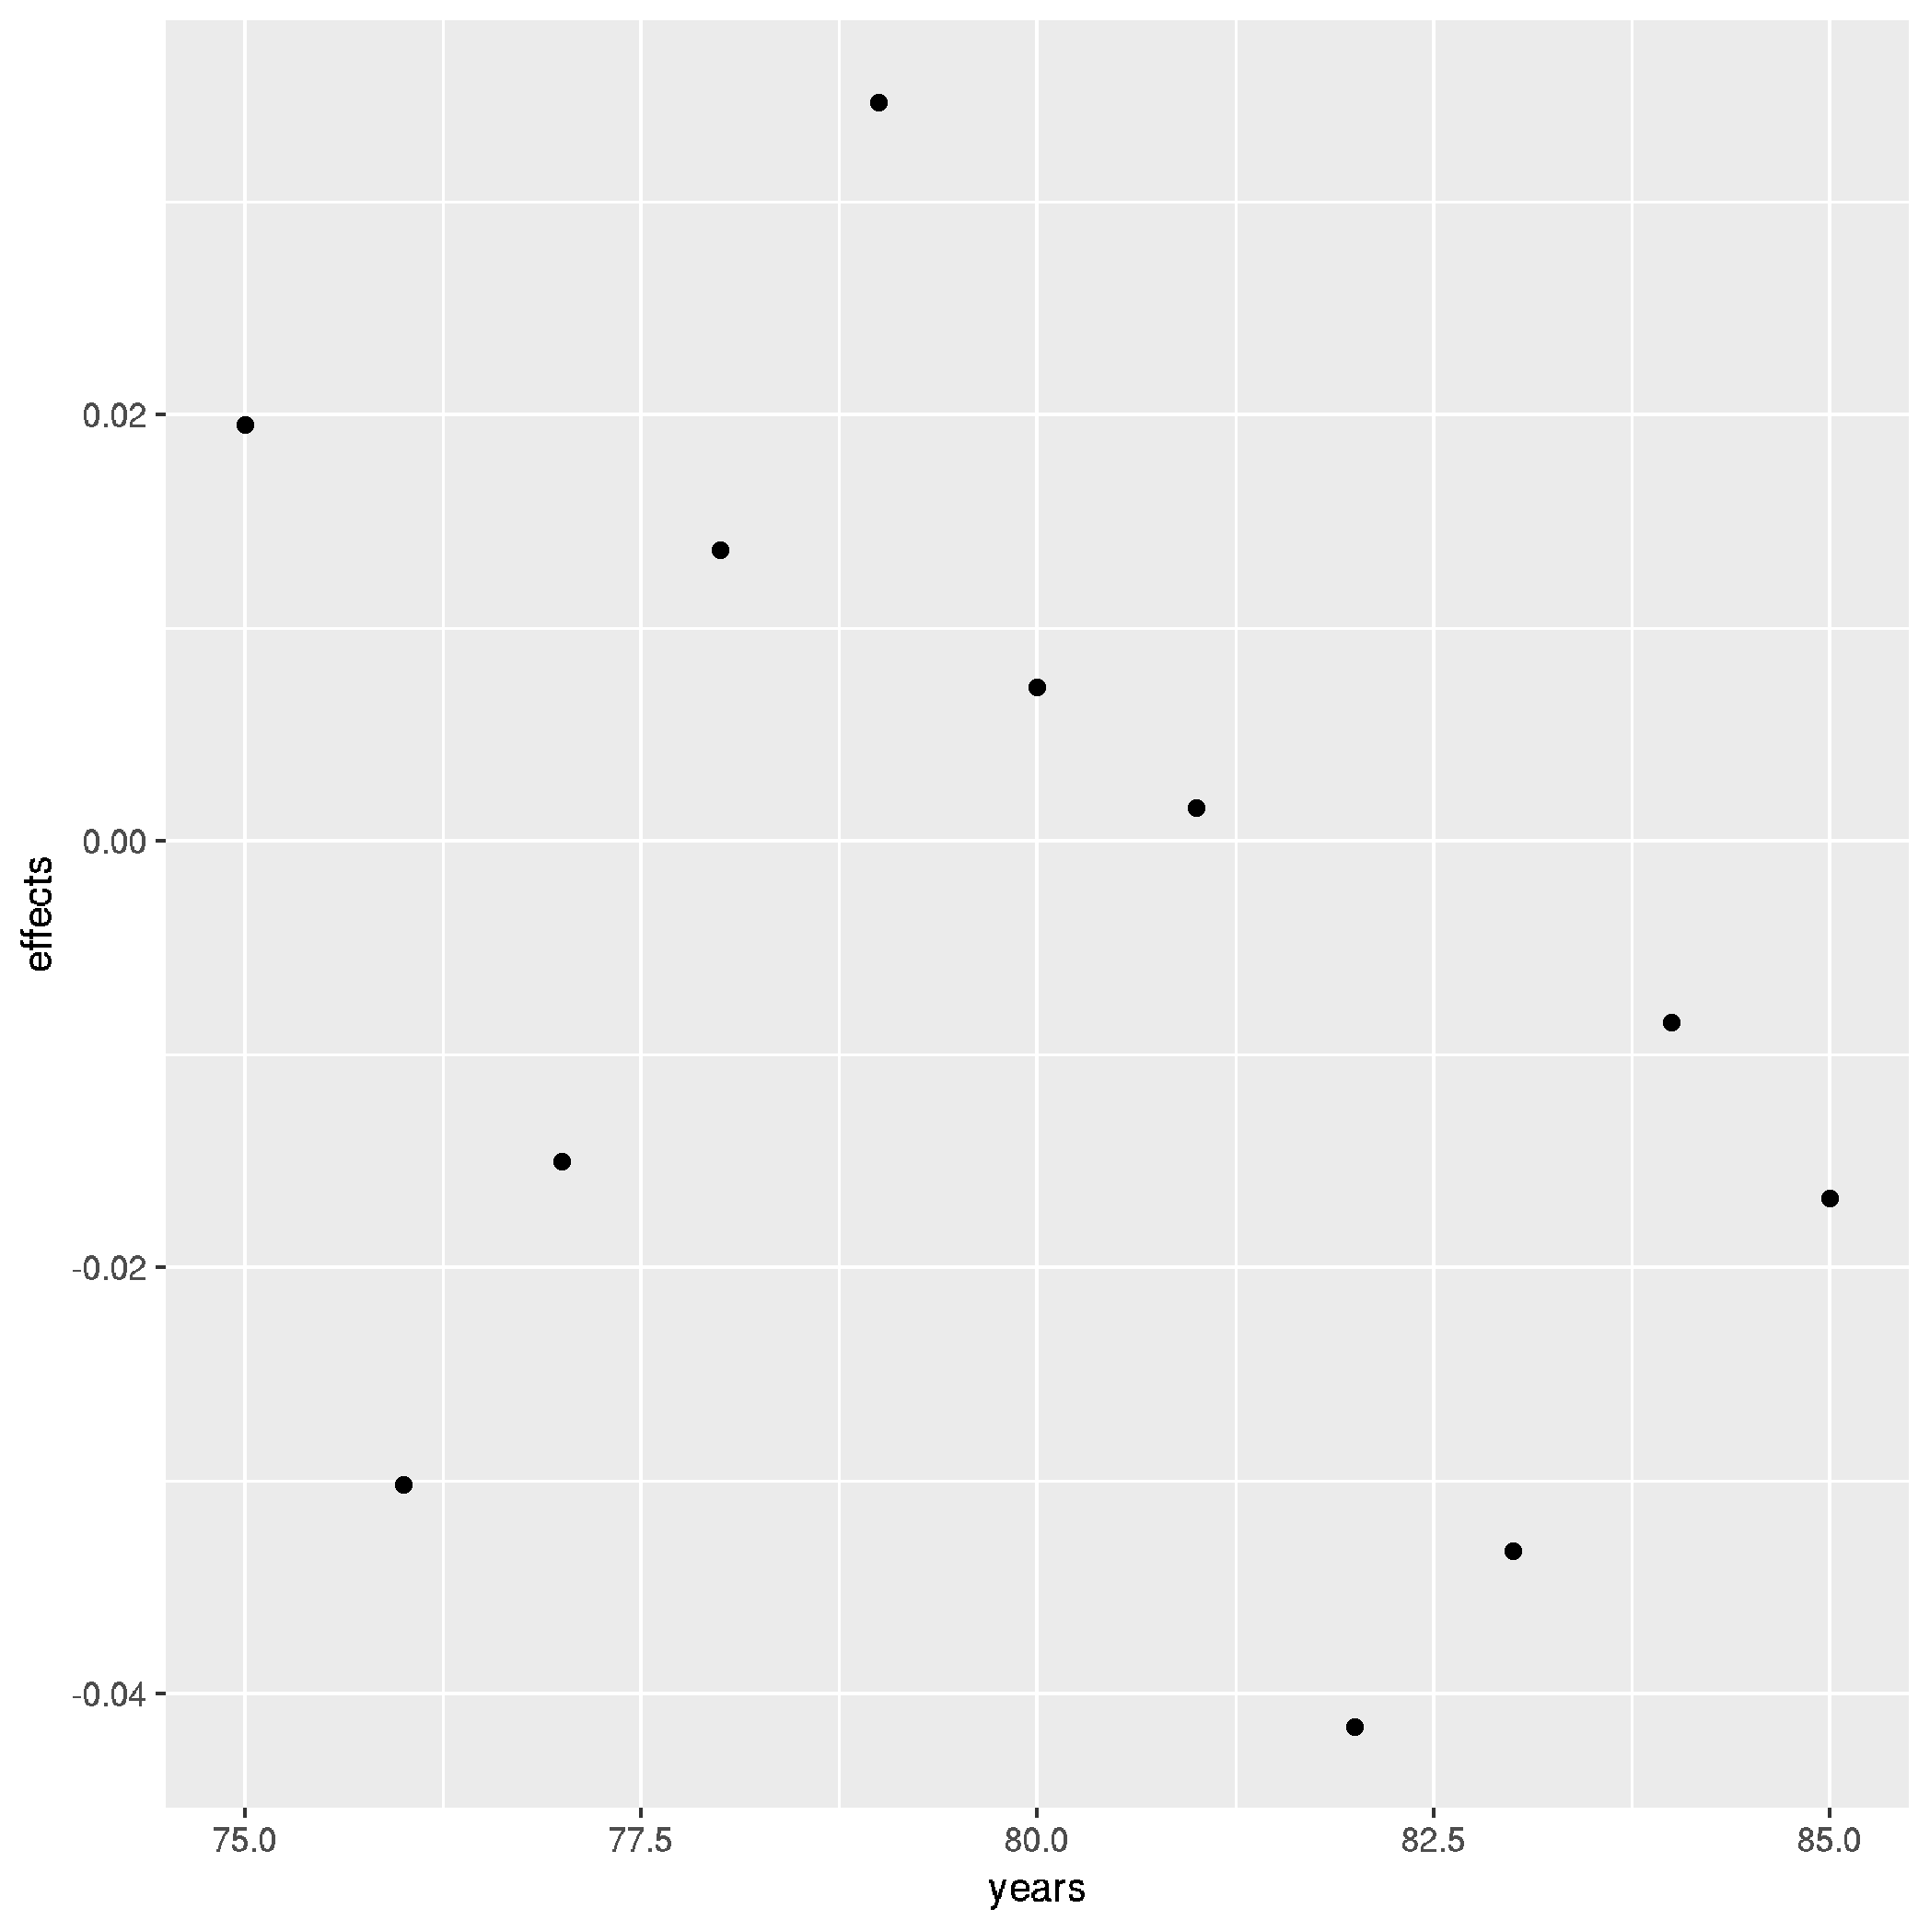
\includegraphics[width=10cm]{time.png}
  \end{center}
\end{figure}
which looks fairly like the average of $ikb$, as expected.

\subsubsection*{c}

This is decently consistent with my knowledge of US economic history. In particular, I don't know any US economic history, so any proposition about it is vacuously true, so I deserve full credit on the question!

More seriously, there were recessions in the US in 1973-1975, as well as 1980 and 1981-1982 (consequences of energy crisis). As I stated above, you would expect in times of recession that investment flows cease, so this graph should show that in those years of recession (with an appropriate time), that the effect is < 0, which is precisely what we see with a large positive effect at the end of the recession in 1975, and a deep trough in the midst of the energy crisis recession in 1982.

\end{document}
% LocalWords:  NetID fancyplain LocalWords colorlinks linkcolor linkbordercolor
